\scanpage{30}
% archive sheet number: 29
% @ drawing / upper half, shaded patch, projection, and two enclosed formulas
\figure{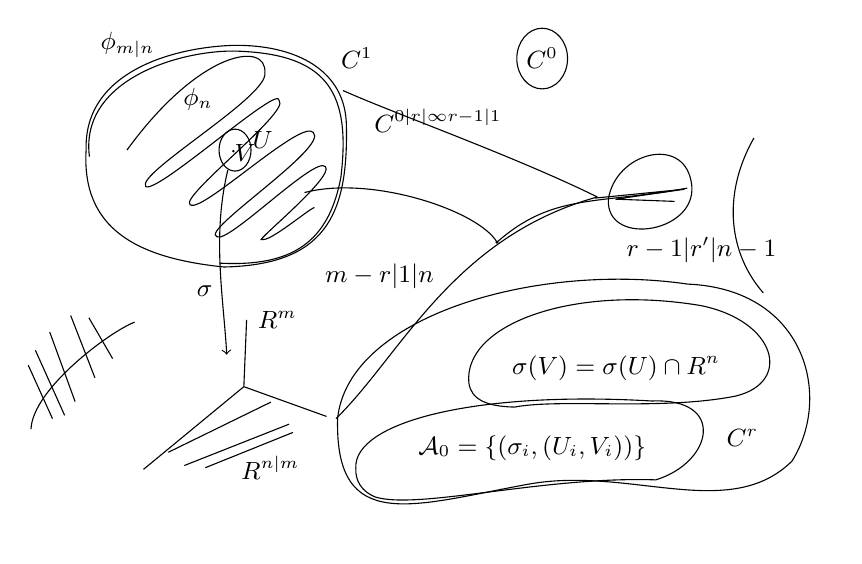
\begin{tikzpicture}[x=.007cm,y=-.007cm,every node/.style={inner sep=1pt,font=\small}]
\draw (313,277) .. controls (309,136) and (471,91) .. (582,88) .. controls (692,87) and (785,132) .. (785,236) .. controls (788,398) and (745,486) .. (563,490) .. controls (407,474) and (304,422) .. (313,277);
\draw[thin] (319,290) .. controls (300,144) and (500,92) .. (597,99) .. controls (753,107) and (793,177) .. (775,327) .. controls (753,445) and (687,490) .. (555,483);
\draw (387,278) .. controls (520,95) and (642,80) .. (637,138) .. controls (645,180) and (403,320) .. (421,344) .. controls (441,359) and (665,156) .. (663,188) .. controls (686,209) and (455,383) .. (508,378) .. controls (545,372) and (705,222) .. (725,246) .. controls (754,273) and (518,425) .. (550,435) .. controls (570,449) and (729,287) .. (747,308) .. controls (764,326) and (614,448) .. (632,440) .. controls (646,445) and (714,387) .. (727,382);
\draw (583,278) ellipse (29 and 38);
\fill (580,280) circle (2.5);
\node at (601,283) {$V$}; \node at (633,259) {$U$};
\node at (388,88) {$\phi_{\unsure{m|n}}$}; \node at (516,186) {$\phi_n$};
\node at (804,111) {$C^1$}; \node at (951,225) {$C^{\deleted{\unsure{0|r|\infty}}\unsure{r-1|1}}$};
\draw (1140,112) ellipse (46 and 55); \node at (1140,111) {$C^0$}; \node at (1266,132) {$\varnothing$};
\draw (709,355) .. controls (831,323) and (1025,388) .. (1058,445);
\fill (1058,445) circle (3); \draw (1058,445) .. controls (1159,356) and (1237,377) .. (1403,347);
\draw (766,765) .. controls (884,650) and (977,436) .. (1240,363);
\draw[thin] (779,170) .. controls (865,209) and (1090,289) .. (1240,363);
\draw (1260,367) .. controls (1273,283) and (1394,251) .. (1410,334) .. controls (1430,427) and (1255,457) .. (1260,367);
\draw (1236,365)--(1398,349)--(1273,367)--(1380,371); \draw (1524,256) .. controls (1465,360) and (1479,466) .. (1541,537); \node at (1429,459) {$\unsure{r-1|r'|n-1}$};
\node at (845,507) {$m-\unsure{r|1|n}$};
\draw[->] (570,314) .. controls (541,434) and (562,544) .. (568,649); \node at (528,534) {$\sigma$};
\draw (604,586)--(599,707)--(749,761); \draw (599,707)--(417,857);
\draw (462,826)--(648,735) (491,850)--(681,775) (529,854)--(688,790);
\node at (660,586) {$R^m$}; \node at (647,854) {$R^{\unsure{n|m}}$};
\draw[thin] (213,784) .. controls (216,711) and (356,607) .. (401,590);
\draw[thin] (208,668)--(252,765) (221,641)--(274,759) (247,608)--(293,734) (285,578)--(329,691) (318,582)--(361,656);
\draw (769,765) .. controls (788,578) and (1132,481) .. (1404,521) .. controls (1617,530) and (1667,724) .. (1593,842) .. controls (1479,954) and (1299,850) .. (1114,884) .. controls (906,922) and (764,976) .. (769,765);
\draw[thin] (1007,700) .. controls (997,594) and (1196,521) .. (1428,560) .. controls (1565,588) and (1594,699) .. (1491,724) .. controls (1355,751) and (1174,728) .. (1090,744) .. controls (1039,743) and (1011,730) .. (1007,700);
\node at (1274,673) {$\sigma(V)=\sigma(U)\cap R^n$};
\draw[thin] (802,855) .. controls (797,772) and (1016,714) .. (1339,733) .. controls (1474,727) and (1450,844) .. (1346,876) .. controls (1143,869) and (915,931) .. (837,907) .. controls (813,897) and (801,878) .. (802,855);
\node at (1122,818) {$\mathcal A_0=\{(\sigma_i,(U_i,V_i))\}$}; \node at (1503,800) {$C^r$};
\end{tikzpicture}}
% @ text / list of four families with right brace on its last two lines
\[
\begin{aligned}
&\boxed{1)\ \text{Familles canoniques}\quad C^r,\ r\geq0} && V_i\subset U_i\\
&2)\ \text{Familles régulières (quasi-régulières)},\ C^r,\ r\geq1\\
&\left.\begin{aligned}
3)&\ \text{familles naturelles}, &r\geq1\\
4)&\ \text{familles normales}, &r\geq1
\end{aligned}\right\}\ C^{r-1}
\end{aligned}
\]
% @ display / lower left, encircled pairs and conditions underneath
\[
\begin{aligned}
&\tikz[baseline=(p.base)]{\node[draw,ellipse,inner xsep=4pt,inner ysep=1.2pt] (p) {$(\sigma_1,(U_1,V_1))\qquad(\sigma_2,(U_2,V_2))$};}\\
1)\quad& V_1\cap V_2\neq\varnothing\\
2)\quad&(\sigma'_1,(U_1\cap U_2,V_1\cap V_2))\\
&\underline{(\sigma'_2,(U_1\cap U_2,V_1\cap V_2))}\\
&U_1\cap V_2=V_1\cap V_2\\
&U_2\cap V_1=V_1\cap V_2
\end{aligned}
\]
% @ drawing / lower right, overlapping patches and images under two arrows
\figure{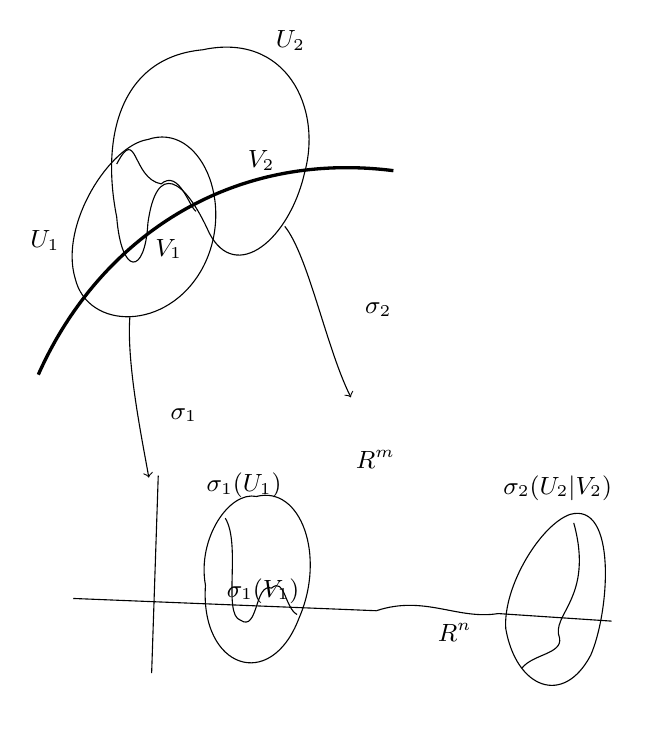
\begin{tikzpicture}[x=.012cm,y=-.012cm,every node/.style={inner sep=1pt,font=\small}]
\draw (1080,1537) .. controls (1063,1480) and (1117,1396) .. (1157,1390) .. controls (1212,1371) and (1251,1458) .. (1215,1526) .. controls (1178,1594) and (1093,1592) .. (1080,1537);
\draw (1124,1472) .. controls (1107,1387) and (1128,1303) .. (1215,1295) .. controls (1303,1276) and (1342,1356) .. (1323,1425) .. controls (1307,1496) and (1250,1543) .. (1222,1489) .. controls (1196,1431) and (1166,1412) .. (1157,1479) .. controls (1154,1534) and (1129,1535) .. (1124,1472);
\draw[very thick] (1041,1639) .. controls (1105,1495) and (1244,1401) .. (1417,1423);
\draw (1124,1416) .. controls (1146,1374) and (1140,1431) .. (1171,1437) .. controls (1190,1421) and (1201,1462) .. (1208,1466);
\node at (1048,1497) {$U_1$};\node at (1308,1285) {$U_2$};\node at (1179,1506) {$V_1$};\node at (1277,1412) {$V_2$};
\draw[->] (1138,1577) .. controls (1134,1628) and (1152,1713) .. (1158,1748);
\draw[->] (1302,1482) .. controls (1327,1513) and (1346,1611) .. (1372,1663);
\node at (1195,1682) {$\sigma_1$};\node at (1401,1570) {$\sigma_2$};
\draw (1168,1746)--(1161,1955) (1078,1876)--(1399,1889) (1528,1892)--(1648,1900);
\draw[thin] (1399,1889)..controls(1450,1872)and(1485,1899)..(1528,1892);
\draw (1218,1862) .. controls (1209,1813) and (1243,1762) .. (1272,1768) .. controls (1319,1756) and (1346,1831) .. (1317,1897) .. controls (1287,1976) and (1212,1950) .. (1218,1862);
\draw (1239,1791) .. controls (1256,1819) and (1236,1893) .. (1255,1899) .. controls (1274,1912) and (1270,1859) .. (1288,1865) .. controls (1302,1853) and (1302,1886) .. (1315,1893);
\draw (1536,1908) .. controls (1533,1863) and (1573,1798) .. (1604,1787) .. controls (1654,1773) and (1646,1890) .. (1626,1936) .. controls (1597,1991) and (1547,1971) .. (1536,1908);
\draw (1608,1796) .. controls (1630,1876) and (1583,1893) .. (1593,1918) .. controls (1596,1935) and (1564,1935) .. (1553,1950);
\node at (1398,1729) {$R^m$};\node at (1482,1912) {$R^n$};
\node at (1259,1756) {$\sigma_1(U_1)$};\node at (1279,1868) {$\sigma_1(V_1)$};\node at (1591,1759) {$\sigma_2(\unsure{U_2|V_2})$};
\end{tikzpicture}}
